\section{Reed-Muller Code}
\label{sec:RMcode}
\lecture{11 Mar.}

As a closing-off to this chapter, let us look at the Reed-Muller code and its similarities with the polar code. This section is highly related to \autoref{sec:w7_RM_RS}.

Consider the encoding of a 2-layer polar code:
\begin{figure}[H]
    \centering
    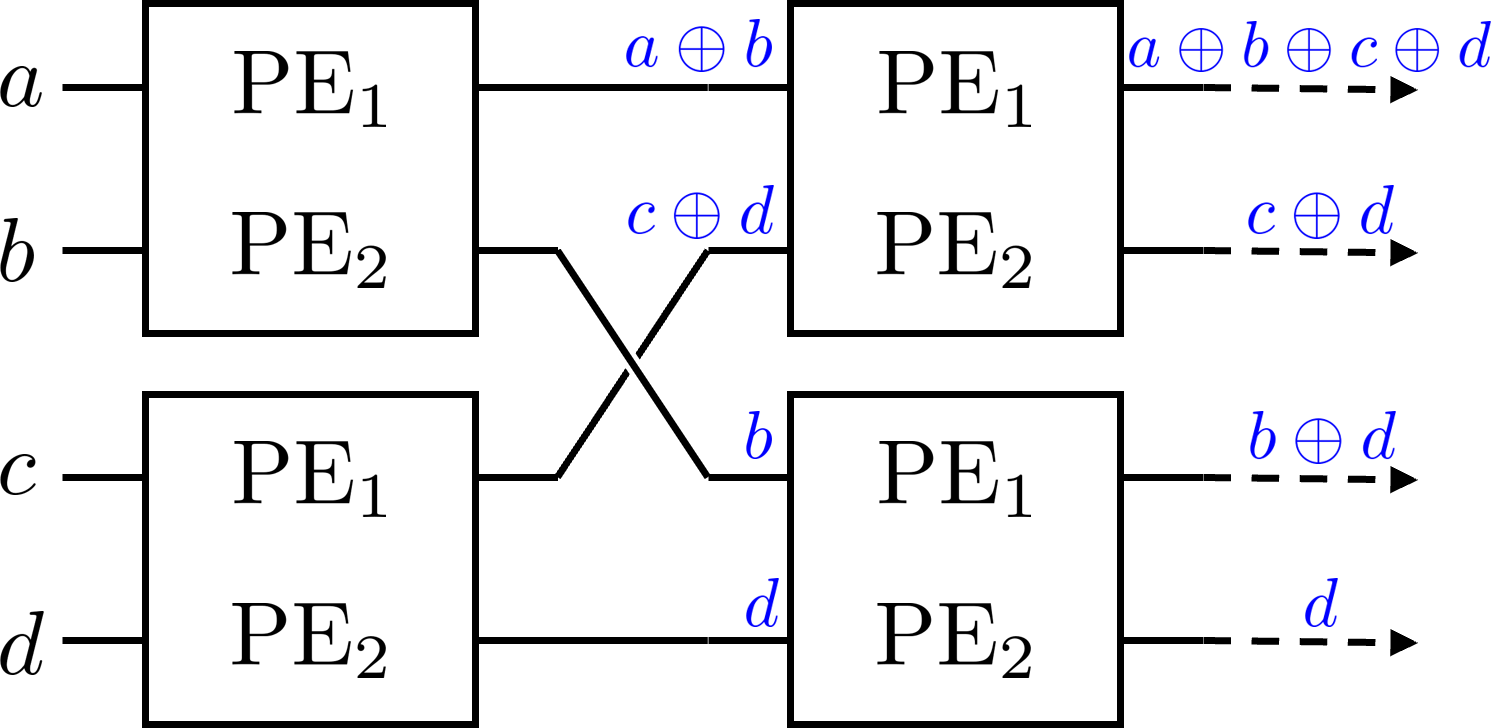
\includegraphics[width=0.4\linewidth]{figures/w4_polar_2layer_enc.png}
    \caption{Codewords of the two-layer polar code.}
\end{figure}
We can rewrite the encoding as a matrix product
\begin{equation}
    \left[\begin{matrix}
        a & c & b & d
    \end{matrix}\right] \left[\begin{matrix}
        1 & 0 & 0 & 0 \\
        1 & 1 & 0 & 0 \\
        1 & 0 & 1 & 0 \\
        1 & 1 & 1 & 1
    \end{matrix}\right] = \left[\begin{matrix}
        a & c & b & d
    \end{matrix}\right] \left[\begin{matrix}
        1 & 0 \\
        1 & 1
    \end{matrix}\right]^{\otimes 2},
\end{equation}
where $\otimes$ is the Kronecker product of matrices.
\begin{definition}[Kronecker Product]
    The Kronecker product of matrices $A= [a_{ij}]$, $B$ is
    \begin{equation}
        A\otimes B = \left[\begin{matrix}
            a_{11} B & a_{12} B & \cdots \\
            a_{21} B & a_{22} B & \cdots \\
            \vdots & \vdots & \ddots
        \end{matrix}\right].
    \end{equation}
    This is also known as the ``tensor product'' of matrices. Note that we also have $A^{\otimes n} = \underbrace{A\otimes \cdots\otimes A}_{n \text{ times}}$.
\end{definition}
In general, under a permutation of the channel orders, we can describe the encoding of an $n$-layer polar code via the matrix
\begin{equation}
    \left[\begin{matrix}
        1 & 0 \\ 1 & 1
    \end{matrix}\right]^{\otimes n},
\end{equation}
this matrix is known as the Ar{\i}kan matrix or the 1011-matrix, which is the \textit{generator matrix} of polar code. By writing out the elements to the Ar{\i}kan matrix explicitly, it beautifully represents the famous fractal \textit{Sierpinski's triangle}. Each row to the Ar{\i}kan's matrix represents a channel $W^s$, where $s\in\{0,1\}^{2^n}$.

Now, how will this help us with the analysis of the code? Recall our scheme for polar code encoding with genie, and compare with the following scheme for Reed-Muller code proposed.
\begin{itemize}
    \item \textbf{Polar Code Encoding:} choose rows of the Ar{\i}kan's matrix with lower $P_e(\mathrm{BEC}(x)^s)$ by applying $f(x)=x^2$ and $g(x)=2x-x^2$ recursively. A partial ordering is created by ordering the error probability.
    \item \textbf{Reed-Muller Code:} choose rows of the Ar{\i}kan's matrix with a lot of $1$'s. Explicitly, choose those with the higher Hamming weights.
\end{itemize}
\begin{example}
    Consider the 3-layer polar code, we have the Ar{\i}kan's matrix with the weights listed as
    \begin{equation*}
        \begin{array}{lc}
            \text{Ar{\i}kan's matrix} & \text{Hamming weight} \\\hline
            1 & 1 \\
            1\;1 & 2 \\
            1\;{\color{lightgray}0}\;1 & 2 \\
            1\;1\;1\;1 & \color{red}4 \\
            1\;{\color{lightgray}0\;0\;0}\;1 & 2 \\
            1\;1\;{\color{lightgray}0\;0}\;1\;1 & \color{red}4 \\
            1\;{\color{lightgray}0}\;1\;{\color{lightgray}0}\;1\;{\color{lightgray}0}\;1 & \color{red}4 \\
            1\;1\;1\;1\;1\;1\;1\;1 & \color{red}8
        \end{array}
    \end{equation*}
    See how those with higher Hamming weights are the ones chosen by the genie! They correspond to those with a lower error probability. Moreover, unlike the analysis of partial ordering over the error probability polynomials. The Hamming weights to $n$-layer polar codes can be easily generalized by doubling the weights to the $(n-1)$-layer polar codes. This is a much simpler ordering scheme when compared to polar code.
\end{example}

The exact amount of rows chosen by the genie to be the good channels under the Reed-Muller code depends on the code rate desired, but the ordering is simply based on the Hamming weights.
\begin{definition}[Reed-Muller Code]
    We define the Reed-Muller code $\mathrm{RM}(r,m)\subseteq\{0,1\}^{2^m}$ as the rows of channels of the Ar{\i}kan's matrix chosen such that their Hamming weights $\ge 2^{m-r}$.
\end{definition}
The higher $r$ is for a given Reed-Muller code $\mathrm{RM}(r,m)$, the higher rate the coding scheme is; on the contrary, for a lower $r$, one pursues a code with high standards.

\begin{remark}
    Some examples to Reed-Muller code listed on Wikipedia are:
    \begin{enumerate}
        \item $\mathrm{RM}(0,m)$: repetition code, 1-dimensional code generate by all-1 vector,
        \item $\mathrm{RM}(m,m)$: the entire space,
        \item $\mathrm{RM}(1,m)$: Hadamard code,
        \item $\mathrm{RM}(m-1,m)$: single-parity-check code,
        \item $\mathrm{RM}(m-2,m)$: extended Hamming code.
    \end{enumerate}
\end{remark}